\section{Communicating Classes}

There are two types of weird Markov chains that we want to avoid. The first one is that when it could essentially be split into many separate Markov chains: when you start in one part of it, you always stay in the same part. \autoref{fig:markov-chain-bad-example-1} shows an example of this, even if the blue edge is included.

\begin{figure}[ht!]
    \centering
    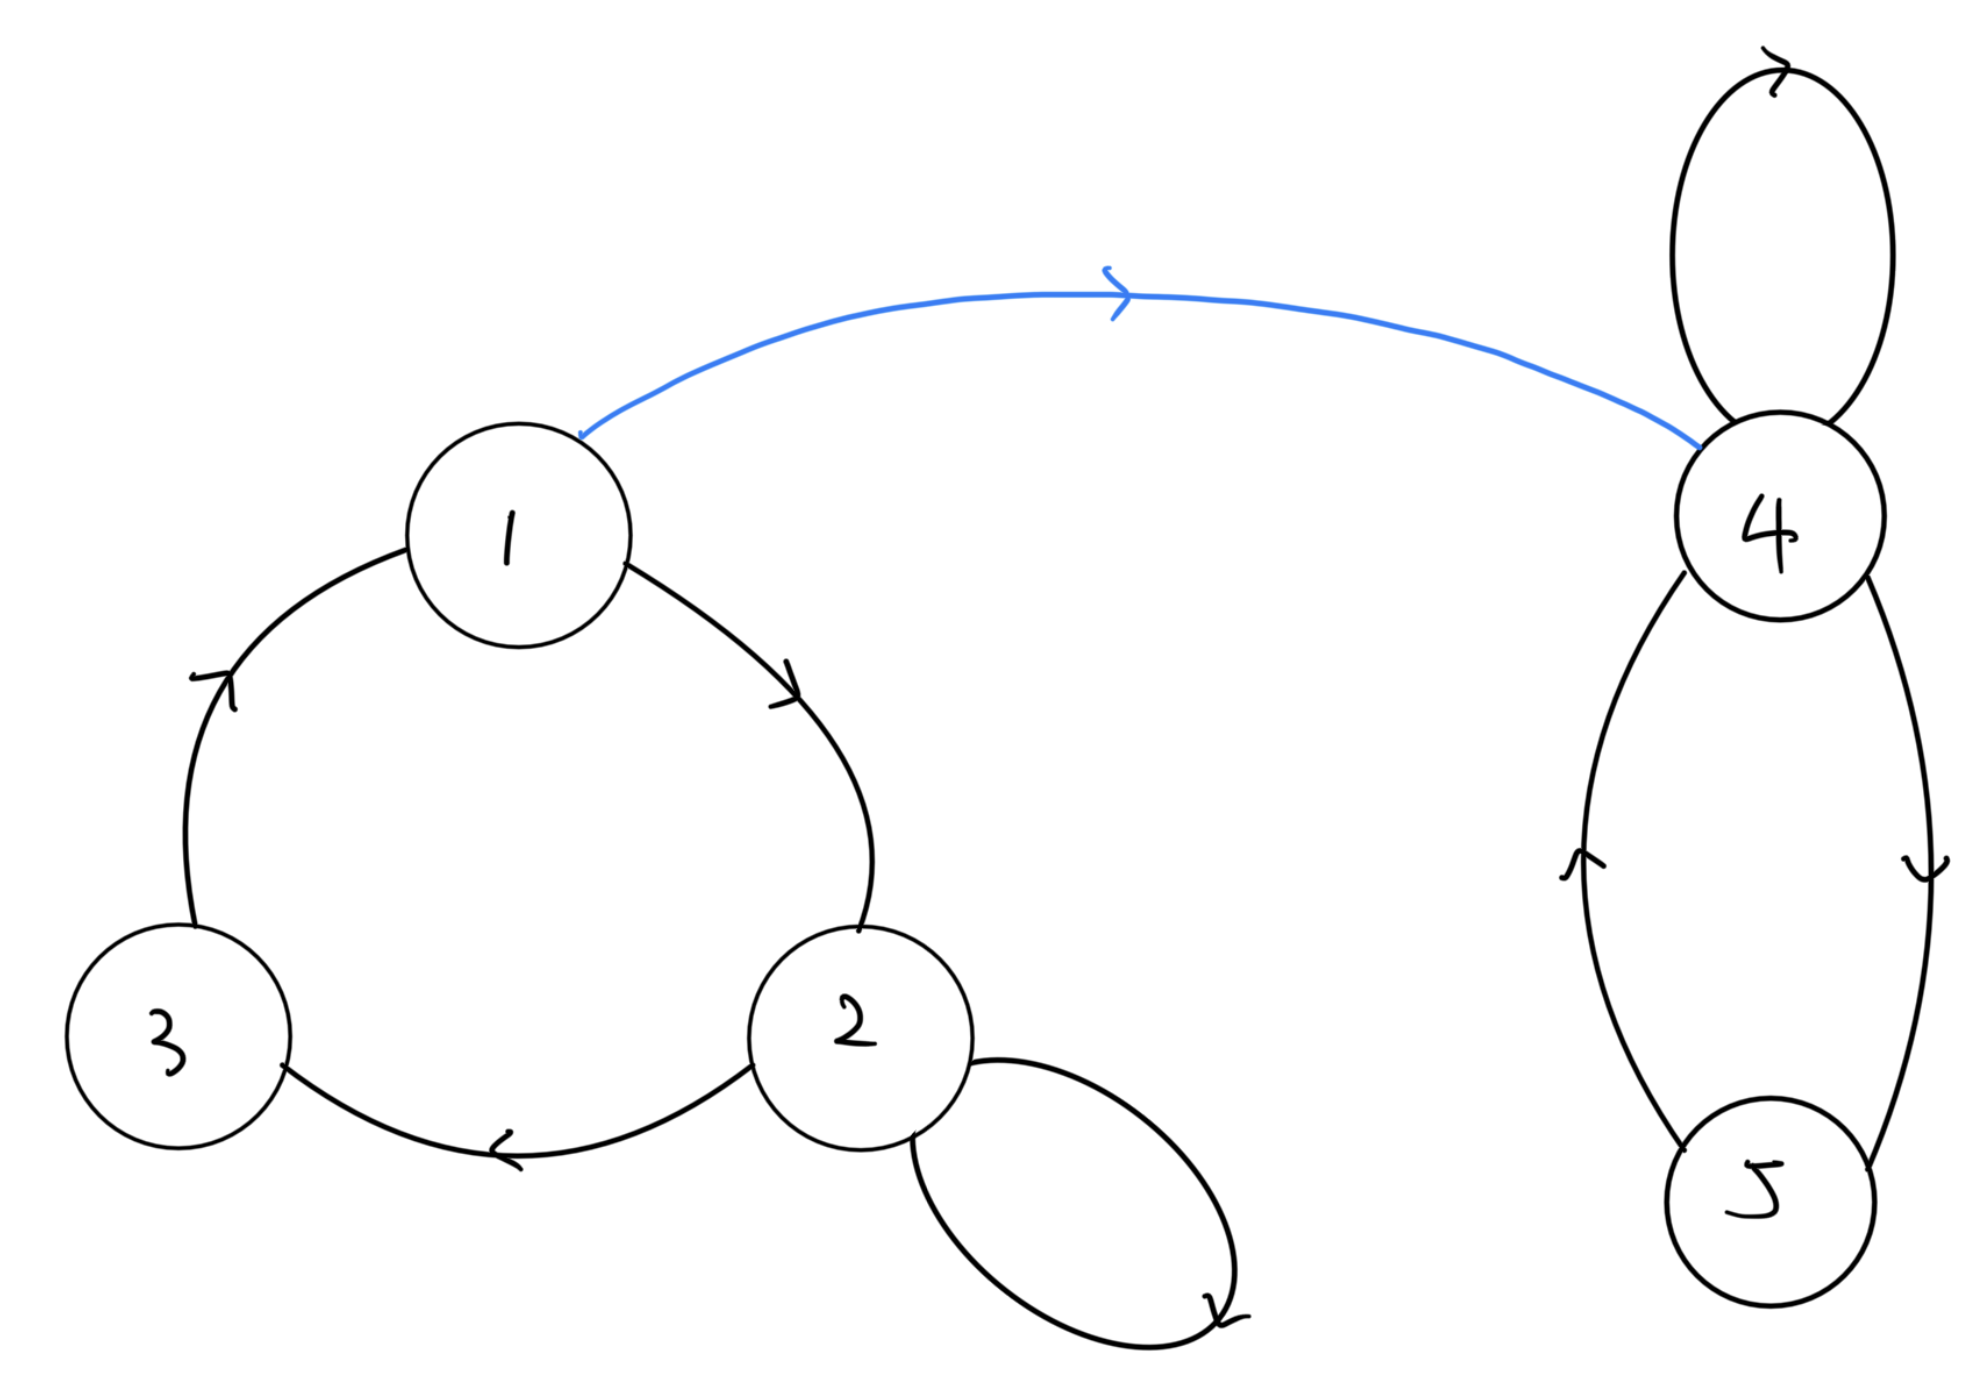
\includegraphics[width=0.7\textwidth]{fig/markov-chain-bad-example-1.png}
    \caption{First Type of ``Weird'' Markov Chains}
    \label{fig:markov-chain-bad-example-1}%
\end{figure}

The second type of weird Markov chains is that certain states have a ``parity'' property. For example, in \autoref{fig:markov-chain-bad-example-2}, if you start at the top-left state, you can only reach the bottom-right state in an even number of steps, and vice versa.

\begin{figure}[ht!]
    \centering
    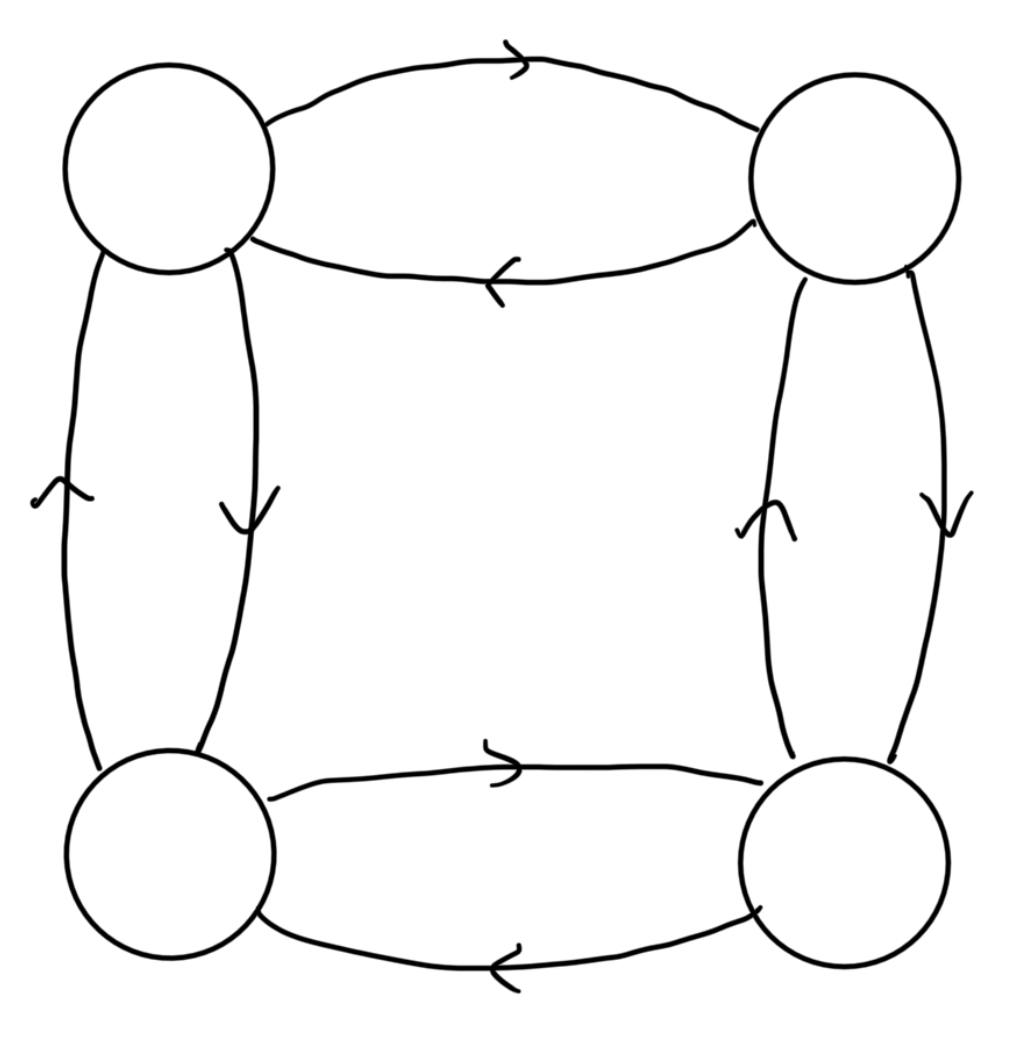
\includegraphics[width=0.4\textwidth]{fig/markov-chain-bad-example-2.png}
    \caption{Second Type of ``Weird'' Markov Chains}
    \label{fig:markov-chain-bad-example-2}%
\end{figure}

\begin{notation}
    We denote
    \begin{align*}
        \Prob_x \pqty{\cdot} = \Prob\pqty{\Conditional{\cdot}{X_0 = x}}, \\
        \Expt_x \pqty{\cdot} = \Expt\pqty{\Conditional{\cdot}{X_0 = x}}.
    \end{align*}    
\end{notation}

\begin{definition}[Leading and Communicating States]
    We say that a state \(x\) \term{leads to} a state \(y\), denoted \(x \leadto y\), if
    \[
        \Prob_x \pqty{X_n = y \text{ for some } n \geq 0} > 0.
    \]

    We say that two states \(x\) and \(y\) \term{communicate}, denoted \(x \communicatewith y\), if \(x \leadto y\) and \(y \leadto x\).
\end{definition}

\begin{theorem}[Characterization of Leading States]
    The following are equivalent.
    
    \begin{enumerate}[label=(\roman*)]
        \item \(x \leadto y\).
        \item There is a sequence of states \(x_0 = x, x_1, x_2, \ldots, x_n = y\) such that \(P_{x_i x_{i + 1}} > 0\) for all \(i = 0, 1, \ldots, n - 1\).
        \item \(\Prob_x \pqty{X_n = y} > 0\) for some \(n \geq 0\).
    \end{enumerate}
\end{theorem}

\begin{proof}
    We note
    \[
        \Bqty{X_n = y \text{ for some } n \geq 0} = \bigcup_{n \geq 0} \Bqty{X_n = y}.
    \]

    This immediately proves the equivalence of (i) and (iii).

    To see that (ii) and (iii) are equivalent, note that
    \begin{align*}
        \Prob+x \pqty{X_n = y} &= \Prob\pqty{\Conditional{X_n = y}{X_0 = x}} \\
        &= \sum_{x_1, x_2, \ldots, x_{n - 1}} \Prob\pqty{\Conditional{X_n = y, X_{n - 1} = x_{n - 1}, \ldots, X_1 = x_1}{X_0 = x}} \\
        &= \sum_{x_1, x_2, \ldots, x_{n - 1}} P_{x x_1} P_{x_1 x_2} \cdots P_{x_{n - 1} y}.
    \end{align*}

    So the left-hand side is positive, which is equivalent to the existence of a sequence of states \(x_0 = x, x_1, x_2, \ldots, x_n = y\) such that \(P_{x_i x_{i + 1}} > 0\) for all \(i = 0, 1, \ldots, n - 1\).
\end{proof}

\begin{corollary}[Communication is an Equivalence Relation]
    Communication is an equvialence relation.
\end{corollary}

\begin{proof}
    First, note \(p_{xx} \pqty{0} = 1\) so \(x \communicatewith x\).

    If \(x \communicatewith y\) and \(y \communicatewith z\), then by previously, taking the paths in the previous theorem, we have \(x \communicatewith z\).

    Finally, if \(x \communicatewith y\), then by definition \(y \communicatewith x\).
\end{proof}

\begin{definition}[Communicating Classes, Closeness, Irreducible, Absorbing States]
    \begin{itemize}
        \item The equivalence classes induced on \(I\) by the relation \(\communicatewith\) are called \term{communicating classes}.

        \item A class \(C \subseteq I\) is \term{closed}, if for any \(x \in C\) and \(y \in I\), that \(x \leadto y\) implies \(y \in C\).

        \item A transition matrix \(P\) of a Markov chain \(X\) is called a \term{irreducible} if there is only one communicating class.
        
        \item A state \(x \in I\) is \term{absorbing} if \(\Bqty{x}\) is a closed class, i.e., \(p_{xx} = 1\pqty{n} = 1\) for all \(n \geq 0\).
    \end{itemize}
\end{definition}